
\chapterbegin{Descripci�n general}
\label{chp:descripcionGeneral}
\minitoc

\section{Esquema General}


\begin{figure}[h]
	\centering
	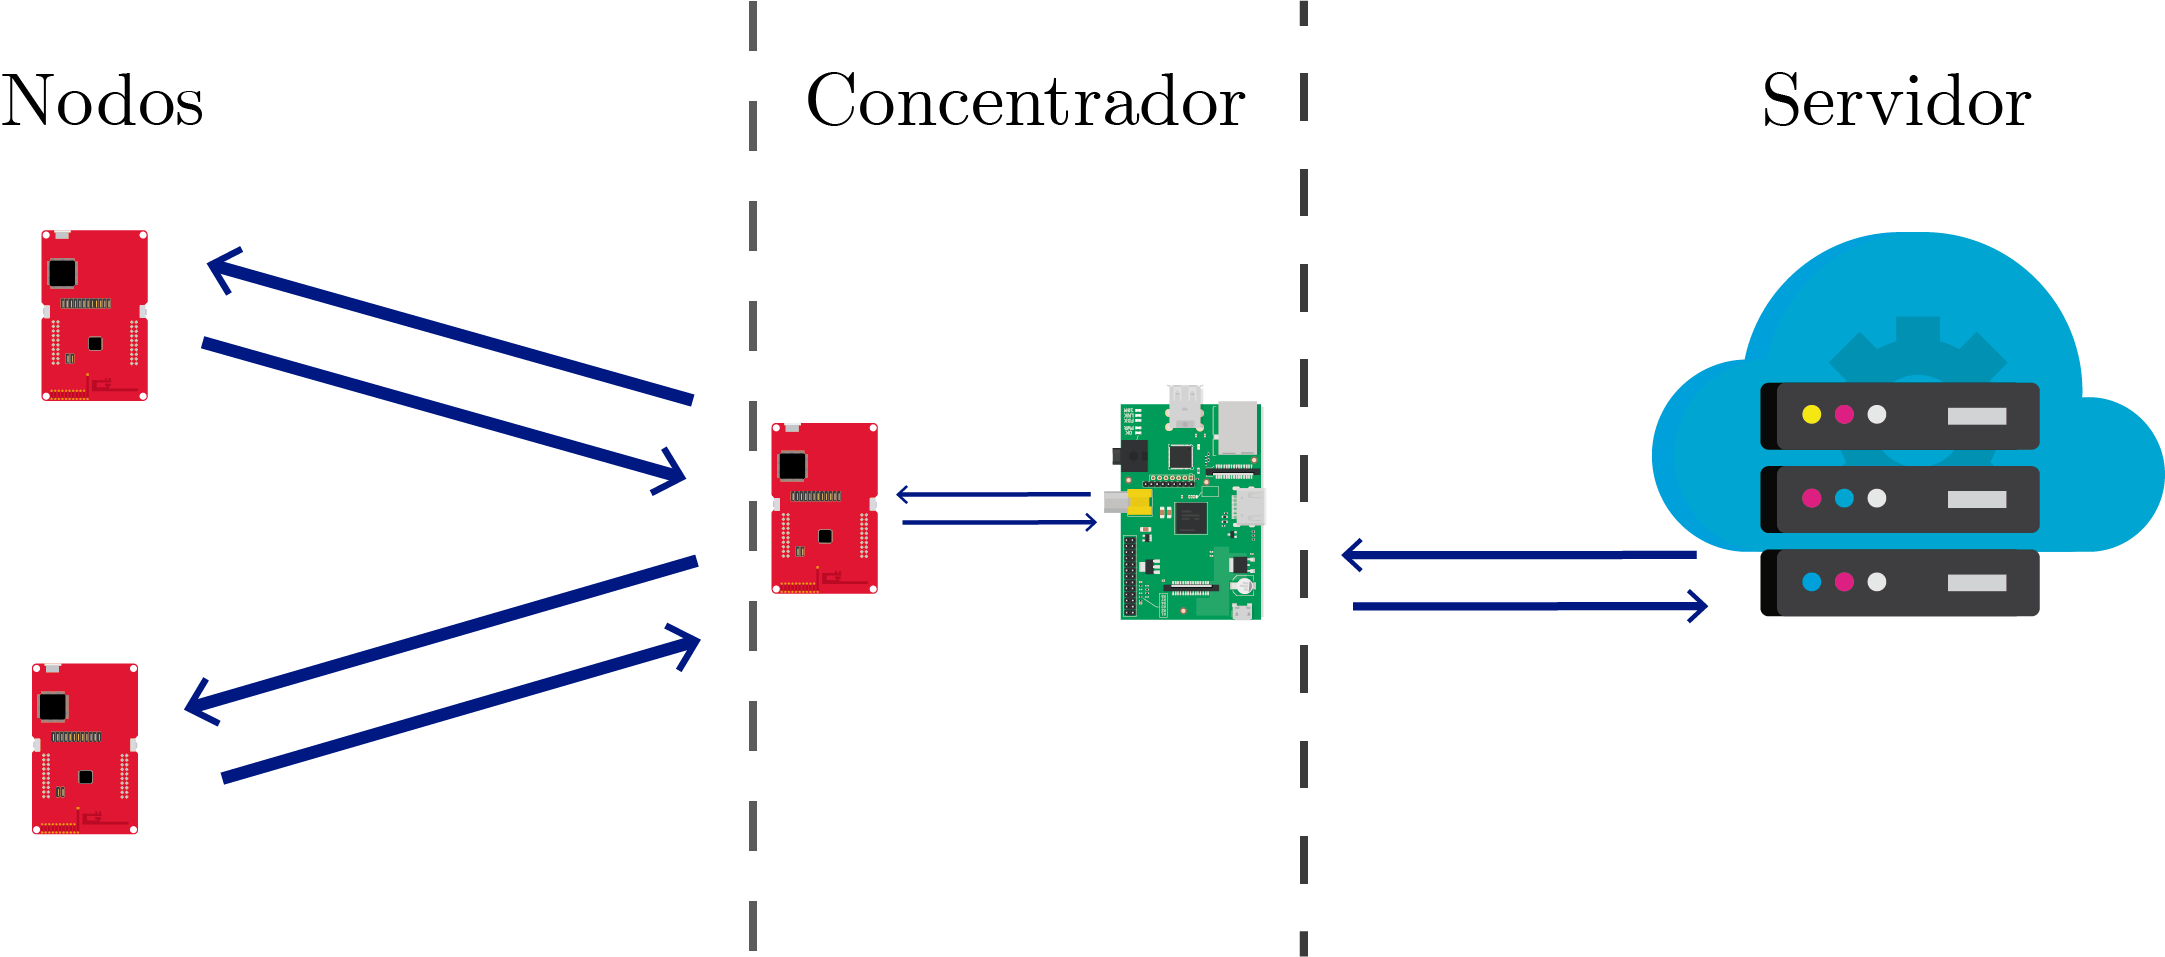
\includegraphics[width=0.8\textwidth]{graphs/DiagramaGeneralTFG}
	\caption{Esquema general del proyecto}
	\label{fig:esquemaGeneral}
\end{figure}

En la figura \ref{fig:esquemaGeneral} se observa el diagrama simplificado de este proyecto donde se est�n representados los diferentes elementos que componen la arquitectura.\\

Del diagrama se extrae que hay cuatro dispositivos distintos: nodo, concentrador, Raspberry Pi y servidor. Cada uno de estos elementos tiene su propia linea de ejecuci�n diferente de los dem�s. Tambi�n se observa como est�n interconectados los diferentes dispositivos usando protocolos diferentes seg�n sea la comunicaci�n. En las siguientes secciones se repasa la funci�n de cada uno de los dispositivos y como se comunican con los dem�s.

\section{Nodo}

El nodo es el extremos de la red, y es el encargado de comunicarle al usuario la \ac{URL} tal y como define la web f�sica. Este est� basado en el microcontrolador CC1350 SimpleLink\TM de Texas Instruments que nos permite comunicaci�n en dos bandas de frecuencia diferentes, en nuestro caso 868MHz y 2.4Ghz.\\

Con el uso de estas dos bandas de frecuencia, el nodo se comunicar� con el usuario usando la banda de 2.4GHz y el protocolo bluetooth. Y con el resto de la red usando la banda de 868MHz y el protocolo TI 15.4 Stack.\\

\section{Concentrador}

El concentrador es el nodo central de la red TI 15.4 Stack, este se encarga de comunicarse con los nodos a 868MHz. Este dispositivo ejecuta un c�digo precompilado, que implementa una capa 802.15.4e/g MAC/PHY y proporciona una interfaz basada en el protocolo \ac{MT} que conecta el dispositivo con el host linux, en nuestro caso una Raspberry Pi.\\

El concentrador est� compuesto por dos dispositivos diferentes, un dispositivo CC1350 que act�a como coprocesador de una RaspberryPi.


\section{Servidor}

El servidor ofrece una interfaz donde es posible administrar la red y enviar comandos a los sensores. Est� compuesto por un servidor NodeJS y una aplicaci�n AngularJS que dan soporte al \textit{Back-end} y \textit{Fron-end}.\\



\chapterend{}